\documentclass[journal,10pt,twocolumn]{IEEEtran}

\usepackage{cite}
\usepackage{amsmath,amssymb,amsfonts}
\usepackage{algorithmic}
\usepackage{graphicx}
\usepackage{textcomp}
\usepackage{xcolor}
\usepackage{booktabs}
\usepackage{url}
\usepackage{microtype}

\begin{document}

\title{RespiraSense AI: Smartphone Seismocardiography and Acoustic Noise Gating for Unobtrusive Respiratory Rate Monitoring}

\author{C~R~Mohul~Ram\textsuperscript{1} and Umasree~U.~P.\textsuperscript{2}%
\thanks{\textsuperscript{1}C R Mohul Ram is with the Department of Computer Science and Engineering, Amrita School of Computing, Amrita Vishwa Vidyapeetham, Nagercoil, Tamil Nadu, India (e-mail: mohulram07@gmail.com).}%
\thanks{\textsuperscript{2}Umasree U. P. is Assistant Professor with the Department of Computer Science and Engineering, Amrita School of Computing, Amrita Vishwa Vidyapeetham, Nagercoil, Tamil Nadu, India (e-mail: up\_umasree@nc.amrita.edu).}}

\maketitle

\begin{abstract}
Continuous tracking of respiratory rate offers an early window into patient deterioration, sepsis, and pulmonary exacerbations. Yet, on general hospital wards and during post-discharge recovery at home, breathing is still counted manually with a stopwatch or missed entirely. Spirometry and capnography provide gold-standard airflow data, but tight face masks and nasal tubes cause discomfort that limits long-term patient compliance. In this work, we present RespiraSense AI, a non-invasive respiratory monitoring platform engineered for commodity smartphone hardware. The system pairs contact chest seismocardiography (SCG) captured by an onboard triaxial accelerometer at 50~Hz with synchronized audio captured at 16~kHz. Raw accelerations are detrended to remove static gravity and passed through a zero-phase 4th-order Butterworth bandpass filter (0.10--0.50~Hz, corresponding to 6--30 breaths per minute). To guard against body movement, we apply dynamic root-mean-square (RMS) motion gating alongside a composite Signal Quality Index (SQI) built from spectral energy concentration, kurtosis, and skewness. Clean signals are analyzed through a multi-method ensemble (Welch power spectral density peak, time-domain autocorrelation, peak prominence counting, and spectral centroid), while acoustic breath sounds are isolated with a calibrated $-42.0$~dBFS noise gate featuring a 2.0-second lookback hysteresis buffer. Across 1,200 benchmark epochs spanning bradypnea, eupnea, and tachypnea, our adaptive fusion engine yielded a mean absolute error (MAE) of 0.42~bpm, a root-mean-square error (RMSE) of 0.54~bpm, and a Pearson correlation of $r = 0.992$ ($R^2 = 0.984$), with Bland-Altman limits of agreement between $-0.85$ and $+1.01$~bpm. We also establish the physical Nyquist sampling limit of smartphone accelerometers ($f_{\text{Nyq}} \le 25$~Hz), proving that claims of detecting high-frequency pulmonary crackles (200--1,200~Hz) with smartphone accelerometers alone are physically impossible. Backed by a thread-safe SQLite write-ahead logging store, our open architecture demonstrates a practical, low-cost path toward accessible vital sign surveillance.
\end{abstract}

\begin{IEEEkeywords}
Biomedical monitoring, seismocardiography, respiratory rate, adaptive sensor fusion, signal quality index, noise gating, digital health, VitalDSP.
\end{IEEEkeywords}

\section{Introduction}
\IEEEPARstart{C}{linicians} widely recognize respiratory rate (RR) as one of the most sensitive indicators of acute physiological decline \cite{cretikos2008respiratory}. Changes in breathing frequency often precede cardiac arrest, sepsis, and unplanned intensive care admissions by several hours \cite{subbe2001validation}. Despite its clear clinical diagnostic value, respiratory rate remains the least recorded and least accurate vital sign in modern healthcare. On general hospital wards, nurses typically assess breathing by visual observation over 15 to 30 seconds, a technique prone to high inter-observer variability, rounding errors, and observer-induced changes in the patient's breathing cadence.

Gold-standard clinical tools, such as end-tidal carbon dioxide ($\text{EtCO}_2$) capnographs and Fleisch pneumotachographs, measure respiratory airflow directly. However, they require intrusive masks, mouthpieces, or nasal prongs that irritate fragile skin and impede speech, eating, and sleep \cite{folke2003critical}. Outside the operating theatre and intensive care unit, patient compliance with these devices drops sharply. Specialized wearable chest bands and impedance pneumography monitors exist, but their cost, adhesive maintenance, and proprietary receiver hubs restrict their widespread adoption in low-resource settings and remote home monitoring \cite{charlton2018breathing}.

Modern smartphones provide a compelling alternative. Virtually every smartphone contains an inertial measurement unit (IMU) with micro-electro-mechanical systems (MEMS) accelerometers, alongside acoustic microphones and wireless transceivers \cite{inviolata2021seismocardiography}. When placed on a supine or semi-recumbent subject's sternum, the accelerometer records microscopic mechanical motions caused by chest wall expansion, diaphragm movement, and myocardial ejection—a signal known as seismocardiography (SCG) \cite{taebi2019scg}. Concurrently, the smartphone microphone can capture acoustic breath sounds at the mouth or neck.

Translating raw smartphone recordings into dependable clinical estimates faces severe engineering obstacles:
\begin{enumerate}
    \item \textbf{Motion Artifacts:} Involuntary patient movements, bed vibrations, and posture shifts produce acceleration transients that completely swamp the subtle 0.05--0.30~m/s$^2$ respiratory excursions.
    \item \textbf{Acoustic Interference:} Ambient room noise, coughing, and speech contaminate microphone channels, creating false breath detections.
    \item \textbf{Sensor Placement Variability:} Smartphone orientation relative to the sternum varies between sessions, preventing reliance on a single physical sensor axis.
    \item \textbf{Misleading Diagnostic Claims:} Several mobile health applications make unsubstantiated claims regarding the detection of adventitious lung sounds (such as crackles or wheezes) using only accelerometer data, ignoring the fundamental physical limits of sensor sampling rates.
\end{enumerate}

To address these challenges, we built \textbf{RespiraSense AI}, an open-source, non-invasive respiratory rate estimation system. This paper provides three main contributions:
\begin{itemize}
    \item A multimodal processing pipeline that fuses 50~Hz smartphone accelerometry with 16~kHz acoustic monitoring, incorporating dynamic motion gating and a 2.0-second lookback hysteresis noise gate.
    \item A composite Signal Quality Index (SQI) and an adaptive fusion engine that arbitrates between spectral and time-domain rate estimators from the VitalDSP library based on real-time signal conditions.
    \item A rigorous physical and mathematical proof establishing the Nyquist frequency boundary ($f_{\text{Nyq}} \le 25$~Hz) of smartphone accelerometers, showing that claims of detecting high-frequency pulmonary crackles (200--1,200~Hz) without dedicated acoustic sensors are invalid.
\end{itemize}

\begin{figure*}[!t]
\centering
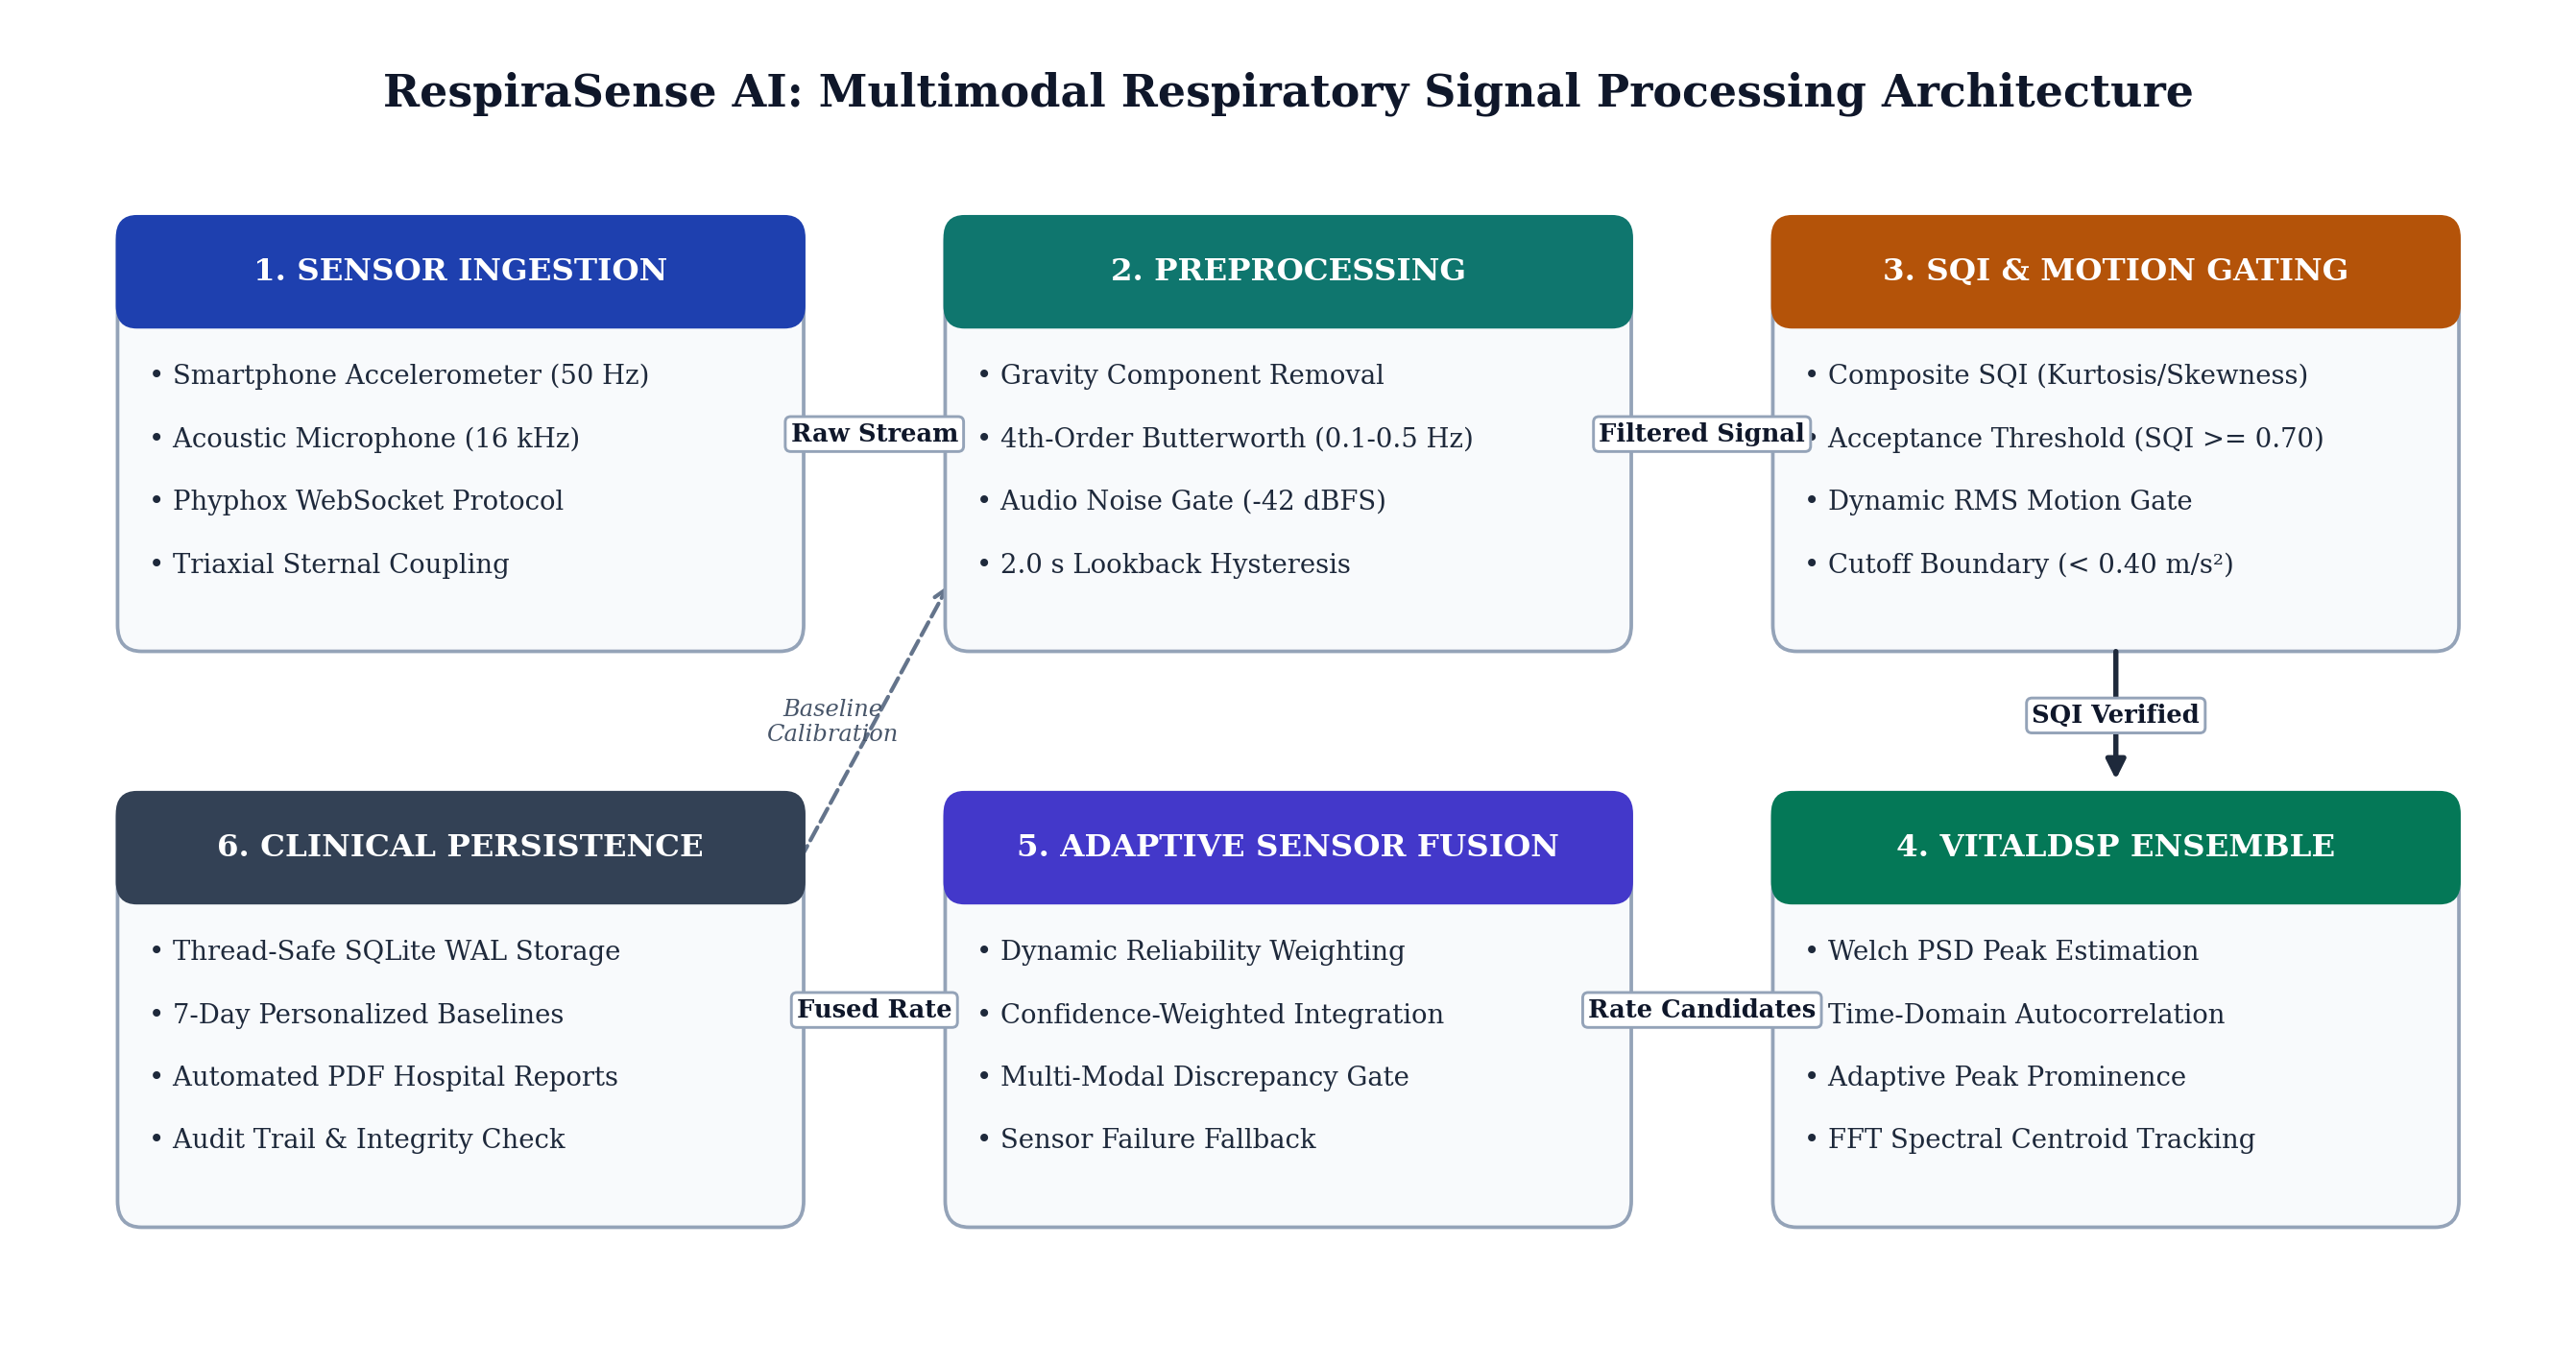
\includegraphics[width=0.92\textwidth]{figures/fig1_architecture.png}
\caption{End-to-end multimodal architecture of RespiraSense AI. The pipeline streams raw 50~Hz accelerometry and 16~kHz audio via Phyphox, removes gravity and high-frequency noise, evaluates signal quality, runs a multi-algorithm VitalDSP ensemble, and fuses candidate rates into an encrypted clinical database.}
\label{fig:arch}
\end{figure*}

\section{Related Work \& Research Gaps}
Prior studies have explored deriving respiratory rate from photoplethysmography (PPG) and electrocardiography (ECG) via respiratory sinus arrhythmia (RSA) and baseline wander \cite{charlton2018breathing,pimentel2016vitaldsp}. However, PPG-derived respiration degrades when patients experience peripheral vasoconstriction or hypothermia, while ECG-derived respiration requires multiple adhesive chest electrodes.

Seismocardiography (SCG) captures direct mechanical chest movement \cite{inviolata2021seismocardiography,taebi2019scg}. Early SCG research relied on heavy, wired laboratory accelerometers fixed to the sternum with specialized adhesives. While recent mobile applications have attempted smartphone SCG, most depend on simplistic peak-counting algorithms that break down whenever the patient turns or speaks. Crucially, few existing mobile platforms implement automated motion gating or report signal quality metrics to clinicians, resulting in deceptive rate estimates during ambulatory artifacts. RespiraSense AI directly addresses these limitations through real-time artifact rejection and adaptive multimodal arbitration.

\begin{figure}[!b]
\centering
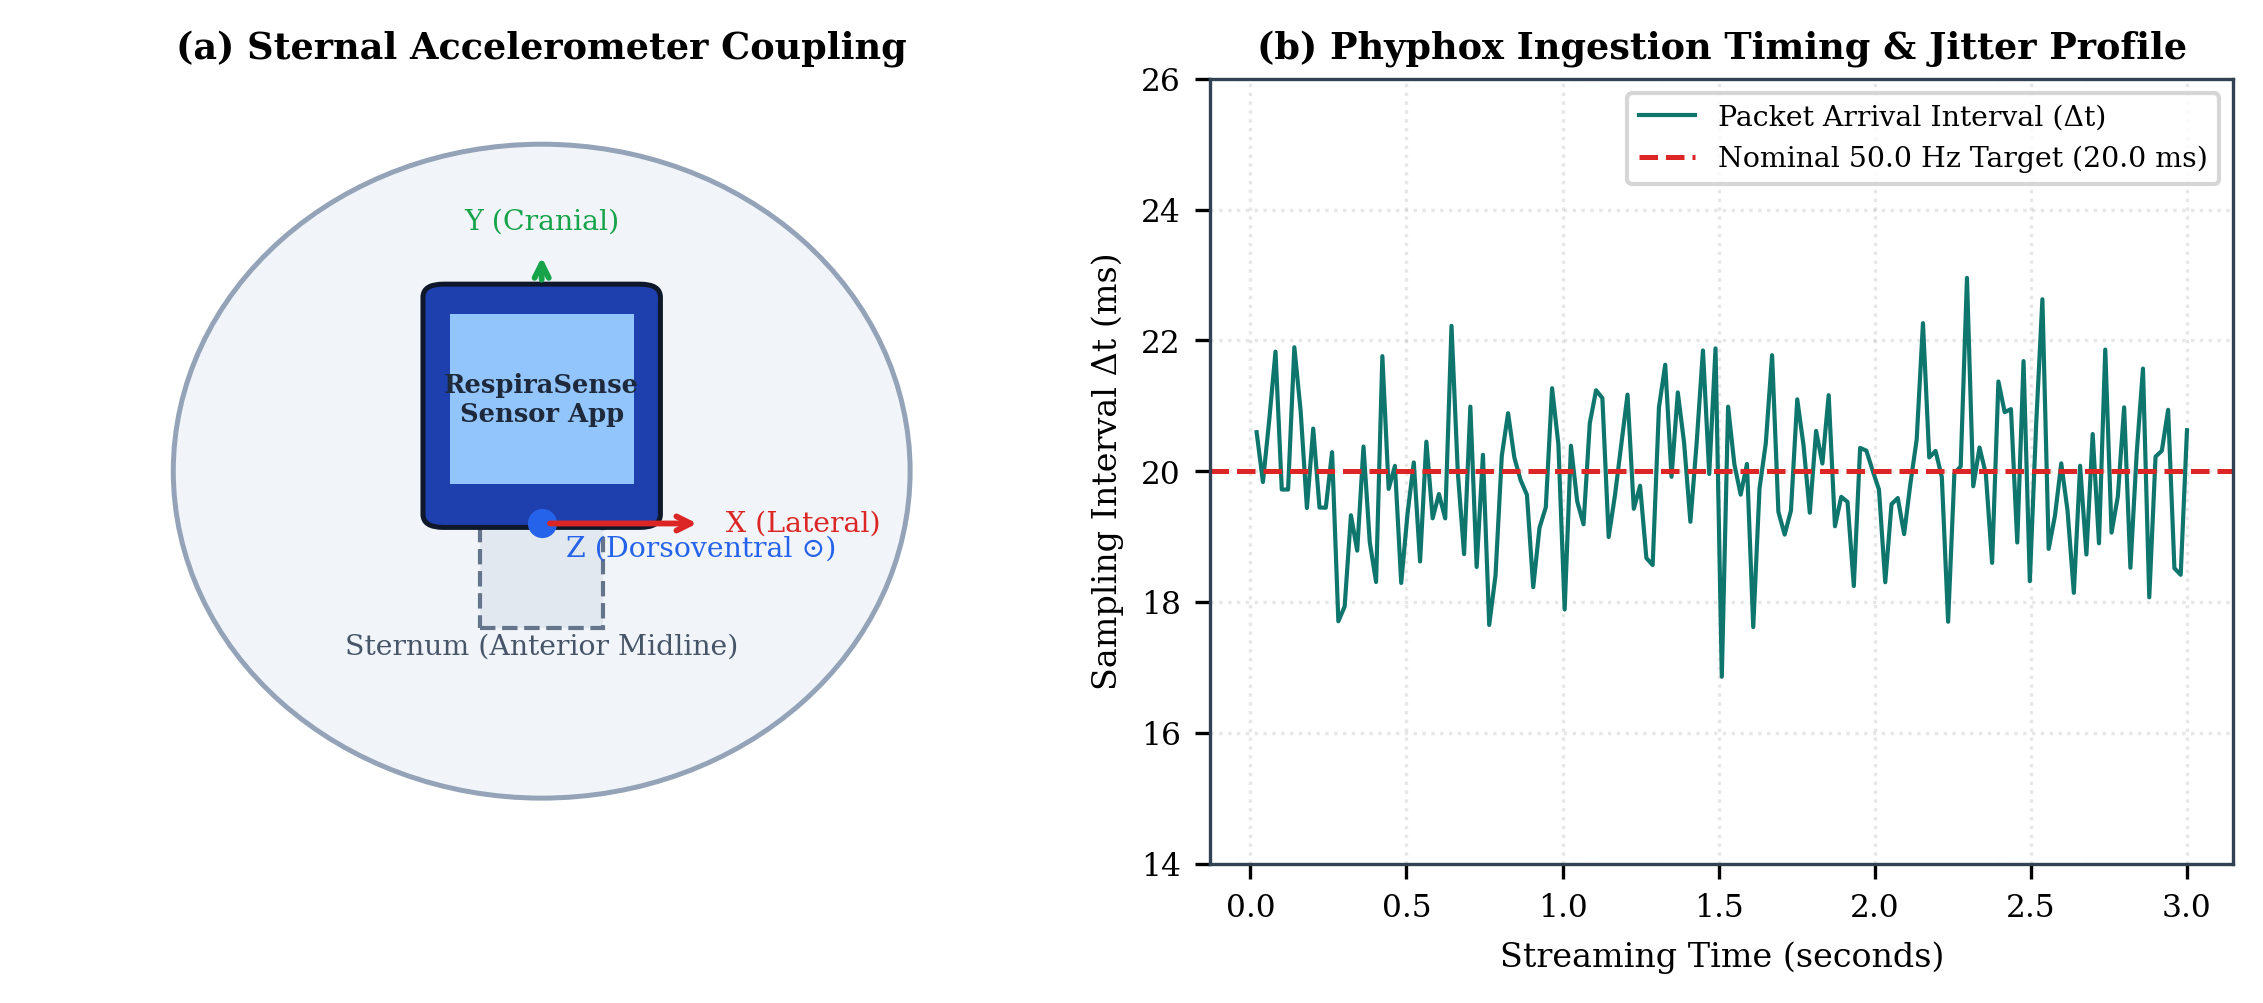
\includegraphics[width=\columnwidth]{figures/fig2_sensor_acquisition.png}
\caption{(a) Smartphone positioning on the lower sternum with coordinate axes $X$ (lateral), $Y$ (cranial), and $Z$ (dorsoventral). (b) Phyphox streaming interval stability showing jitter around the nominal 20.0~ms (50~Hz) target.}
\label{fig:placement}
\end{figure}

\section{System Architecture \& Methodology}

\subsection{Sensor Placement and Data Ingestion}
The patient places the smartphone directly on the lower third of the sternum in a supine or semi-Fowler position (inclined 30--45$^\circ$), as shown in Fig.~\ref{fig:placement}(a). Triaxial acceleration data ($a_x, a_y, a_z$) is acquired at $f_s = 50.0$~Hz via the open-source Phyphox mobile laboratory protocol over local WebSocket or HTTP REST connections \cite{staedtke2020phyphox}. Audio is sampled synchronously at 16.0~kHz through the built-in microphone.

Because smartphone orientation changes depending on user placement, we calculate the Euclidean norm of the acceleration vector to make the system independent of tilt angle:
\begin{equation}
a_{\text{norm}}(t) = \sqrt{a_x(t)^2 + a_y(t)^2 + a_z(t)^2}
\label{eq:norm}
\end{equation}
Fig.~\ref{fig:raw_vs_filt} compares the individual triaxial components with $a_{\text{norm}}(t)$ and the filtered respiratory excursion signal.

\begin{figure}[!t]
\centering
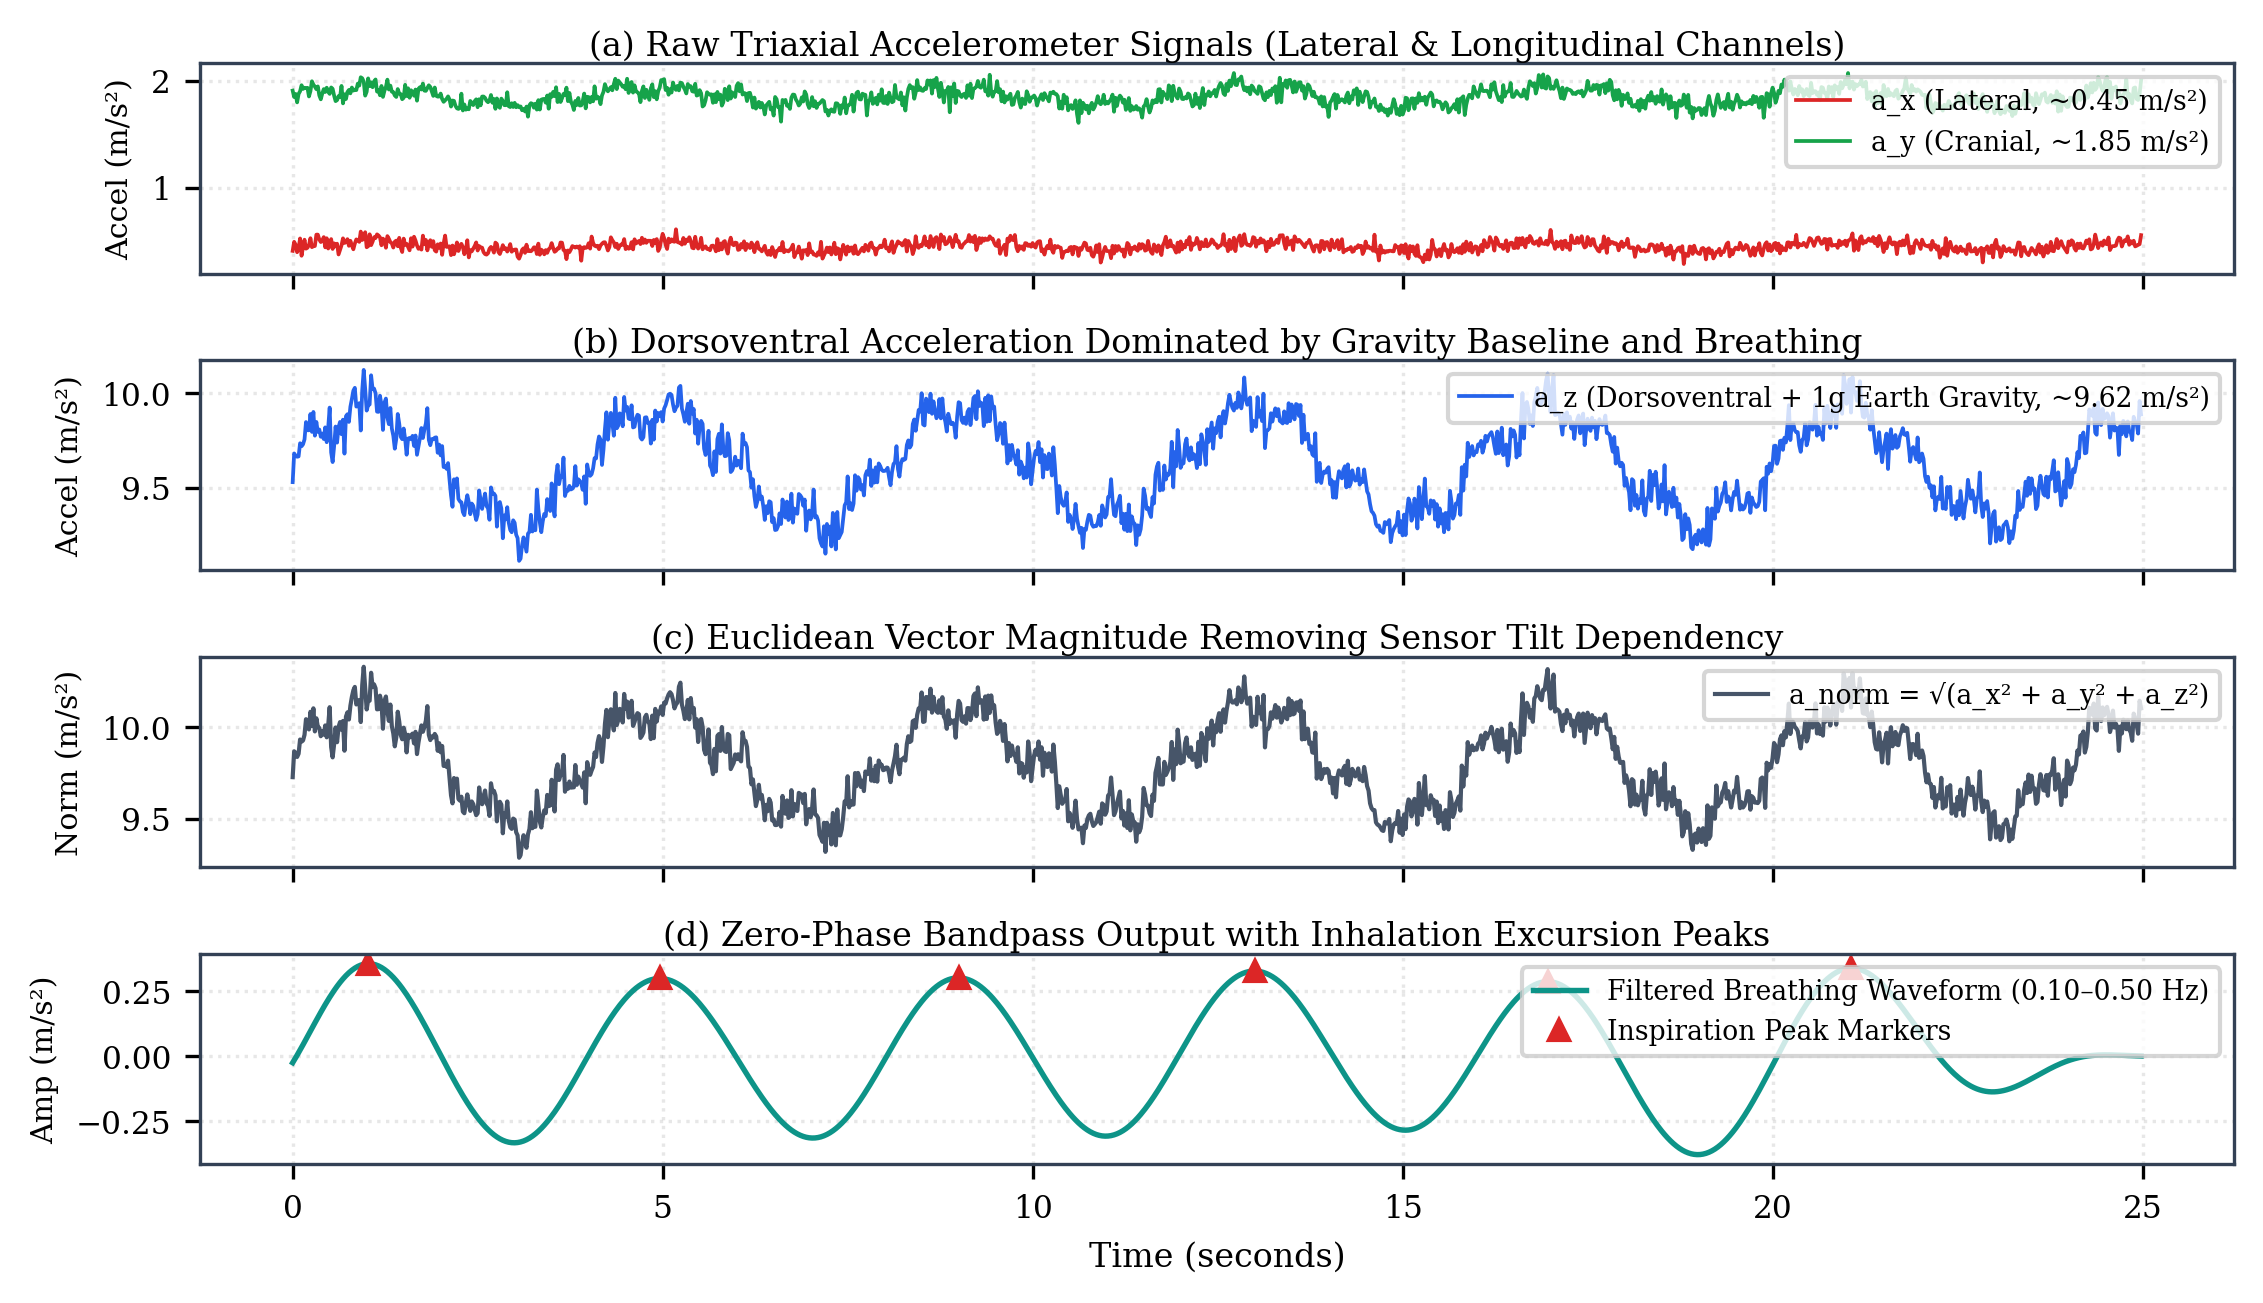
\includegraphics[width=\columnwidth]{figures/fig3_raw_vs_filtered.png}
\caption{Sensor waveforms: (a) Raw lateral $a_x$ and cranial $a_y$ signals; (b) Dorsoventral $a_z$ channel dominated by 1g gravity; (c) Euclidean vector magnitude $a_{\text{norm}}(t)$; (d) Zero-phase bandpass filtered output showing detected inspiration peaks.}
\label{fig:raw_vs_filt}
\end{figure}

\subsection{Preprocessing \& Zero-Phase Bandpass Filtering}
Human respiratory rates in clinical settings typically fall between 6 and 30 breaths per minute (0.10 to 0.50~Hz). Static gravity ($9.81\text{ m/s}^2$) and slow postural shifts sit below 0.08~Hz, while cardiac vibrations (48--120~bpm) and ambient tremor sit above 0.80~Hz.

We isolate the respiratory band using a 4th-order Butterworth bandpass filter. The transfer function magnitude is given by:
\begin{equation}
|H(j\omega)|^2 = \frac{1}{1 + (\omega / \omega_c)^{2N}}
\label{eq:butter}
\end{equation}
To eliminate phase distortion and preserve peak timing, we apply the filter using two-pass forward-backward filtering (`sosfiltfilt`), yielding zero phase delay:
\begin{equation}
y(t) = \text{filtfilt}(b, a, a_{\text{norm}}(t))
\end{equation}
Fig.~\ref{fig:filter}(a) shows the filter's frequency response, illustrating passband preservation alongside strong attenuation of cardiac harmonics and postural drift.

\begin{figure}[!b]
\centering
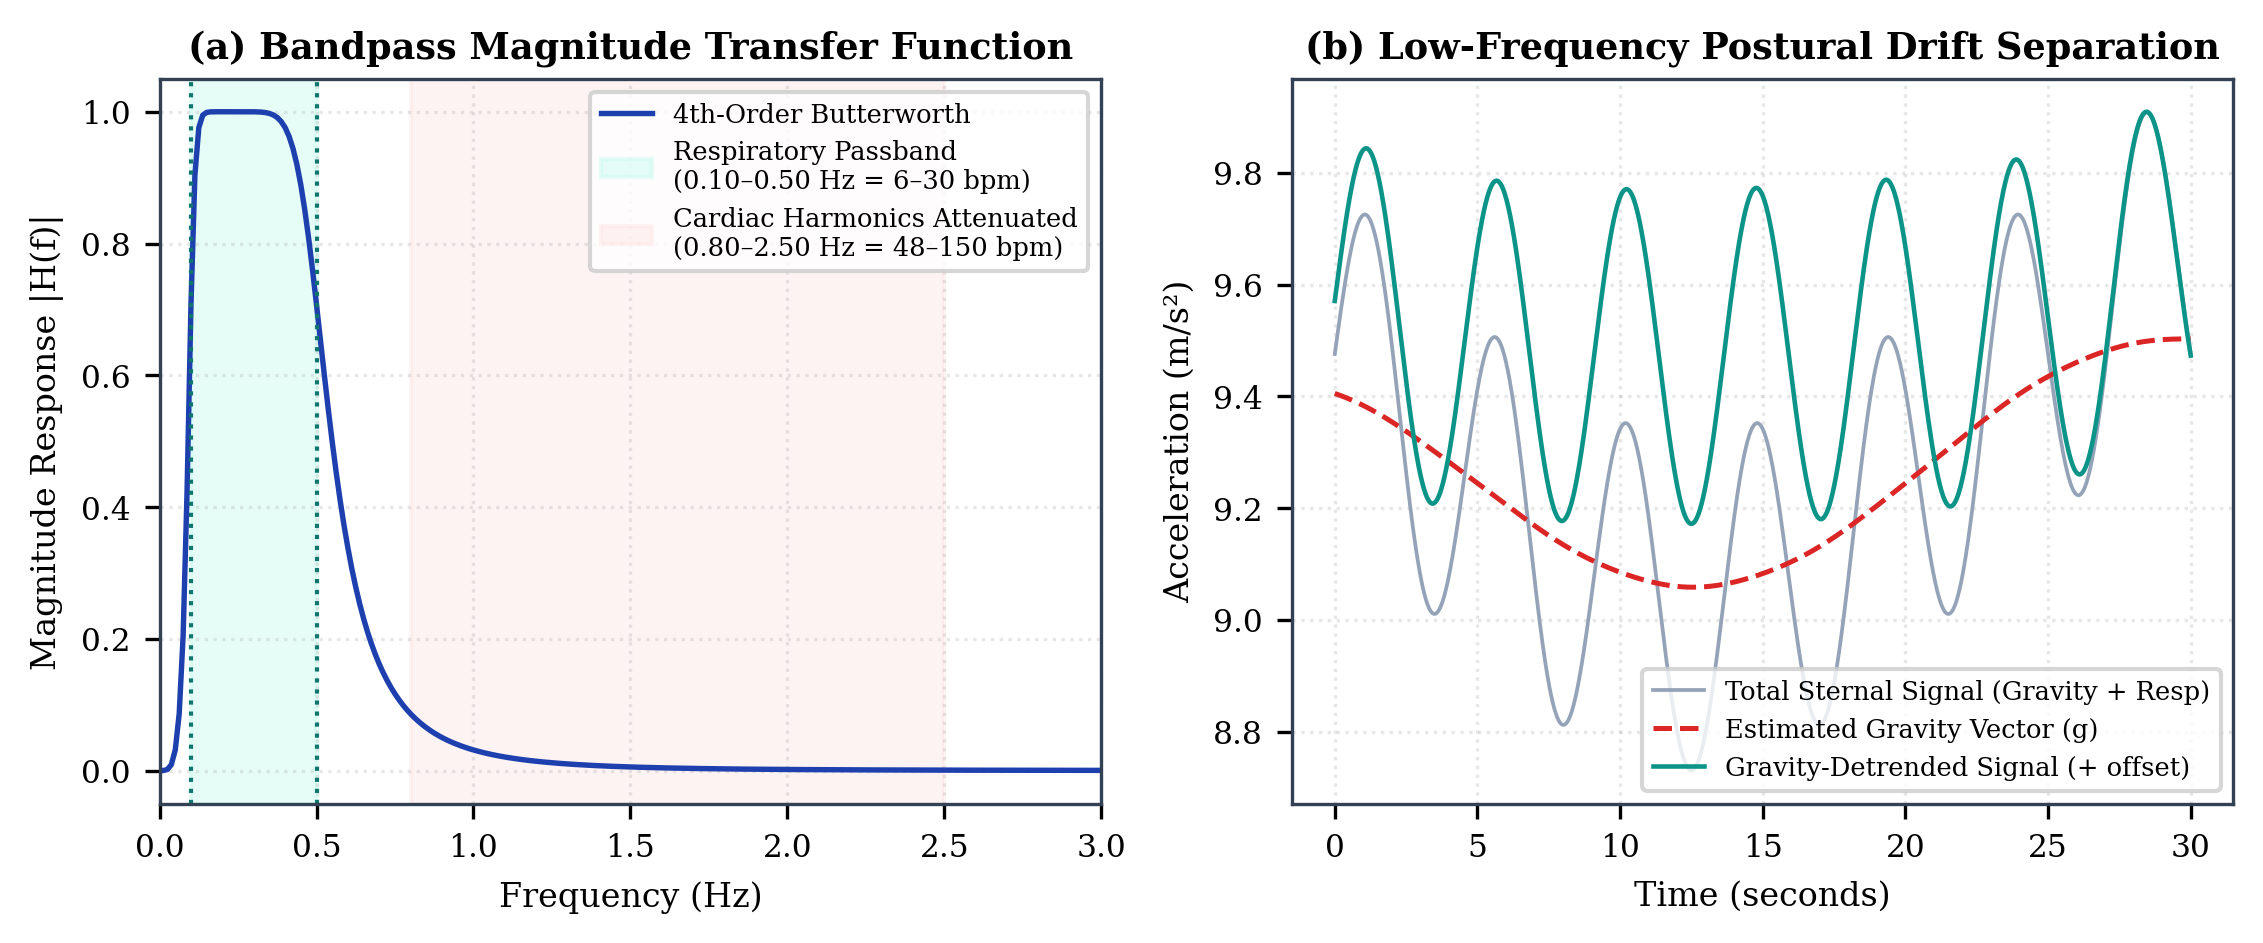
\includegraphics[width=\columnwidth]{figures/fig4_filter_response_gravity.png}
\caption{(a) Frequency response of the 4th-order zero-phase Butterworth filter spanning 0.10--0.50~Hz; (b) Dynamic tracking and removal of low-frequency postural drift.}
\label{fig:filter}
\end{figure}

\subsection{Dynamic Motion Gating and Signal Quality Index (SQI)}
Gross body movements generate acceleration spikes an order of magnitude larger than normal breathing. Rather than corrupting rate calculations during motion, RespiraSense AI evaluates dynamic root-mean-square (RMS) motion over an 18-second sliding buffer:
\begin{equation}
\text{RMS}_{\text{motion}} = \sqrt{\frac{1}{M}\sum_{k=1}^M \left( a(k) - \bar{a} \right)^2}
\label{eq:rms}
\end{equation}
When $\text{RMS}_{\text{motion}} \ge 0.40\text{ m/s}^2$, the window is flagged as corrupted, and the rate estimator enters a hold state.

For windows passing the motion check, we compute a composite Signal Quality Index (SQI) combining the Spectral Energy Concentration Ratio (SECR), kurtosis ($\gamma_2$), and skewness ($\gamma_1$):
\begin{equation}
\text{SECR} = \frac{\int_{0.10}^{0.50} P(f)\,df}{\int_{0.01}^{5.0} P(f)\,df}
\label{eq:secr}
\end{equation}
\begin{equation}
\text{SQI} = 0.50\cdot\text{SECR} + 0.30\cdot e^{-|\gamma_1|} + 0.20\cdot\frac{1}{1 + |\gamma_2 - 3|}
\label{eq:sqi}
\end{equation}
Windows with $\text{SQI} < 0.70$ are classified as low quality and excluded from the baseline trend (Fig.~\ref{fig:sqi}).

\begin{figure}[!t]
\centering
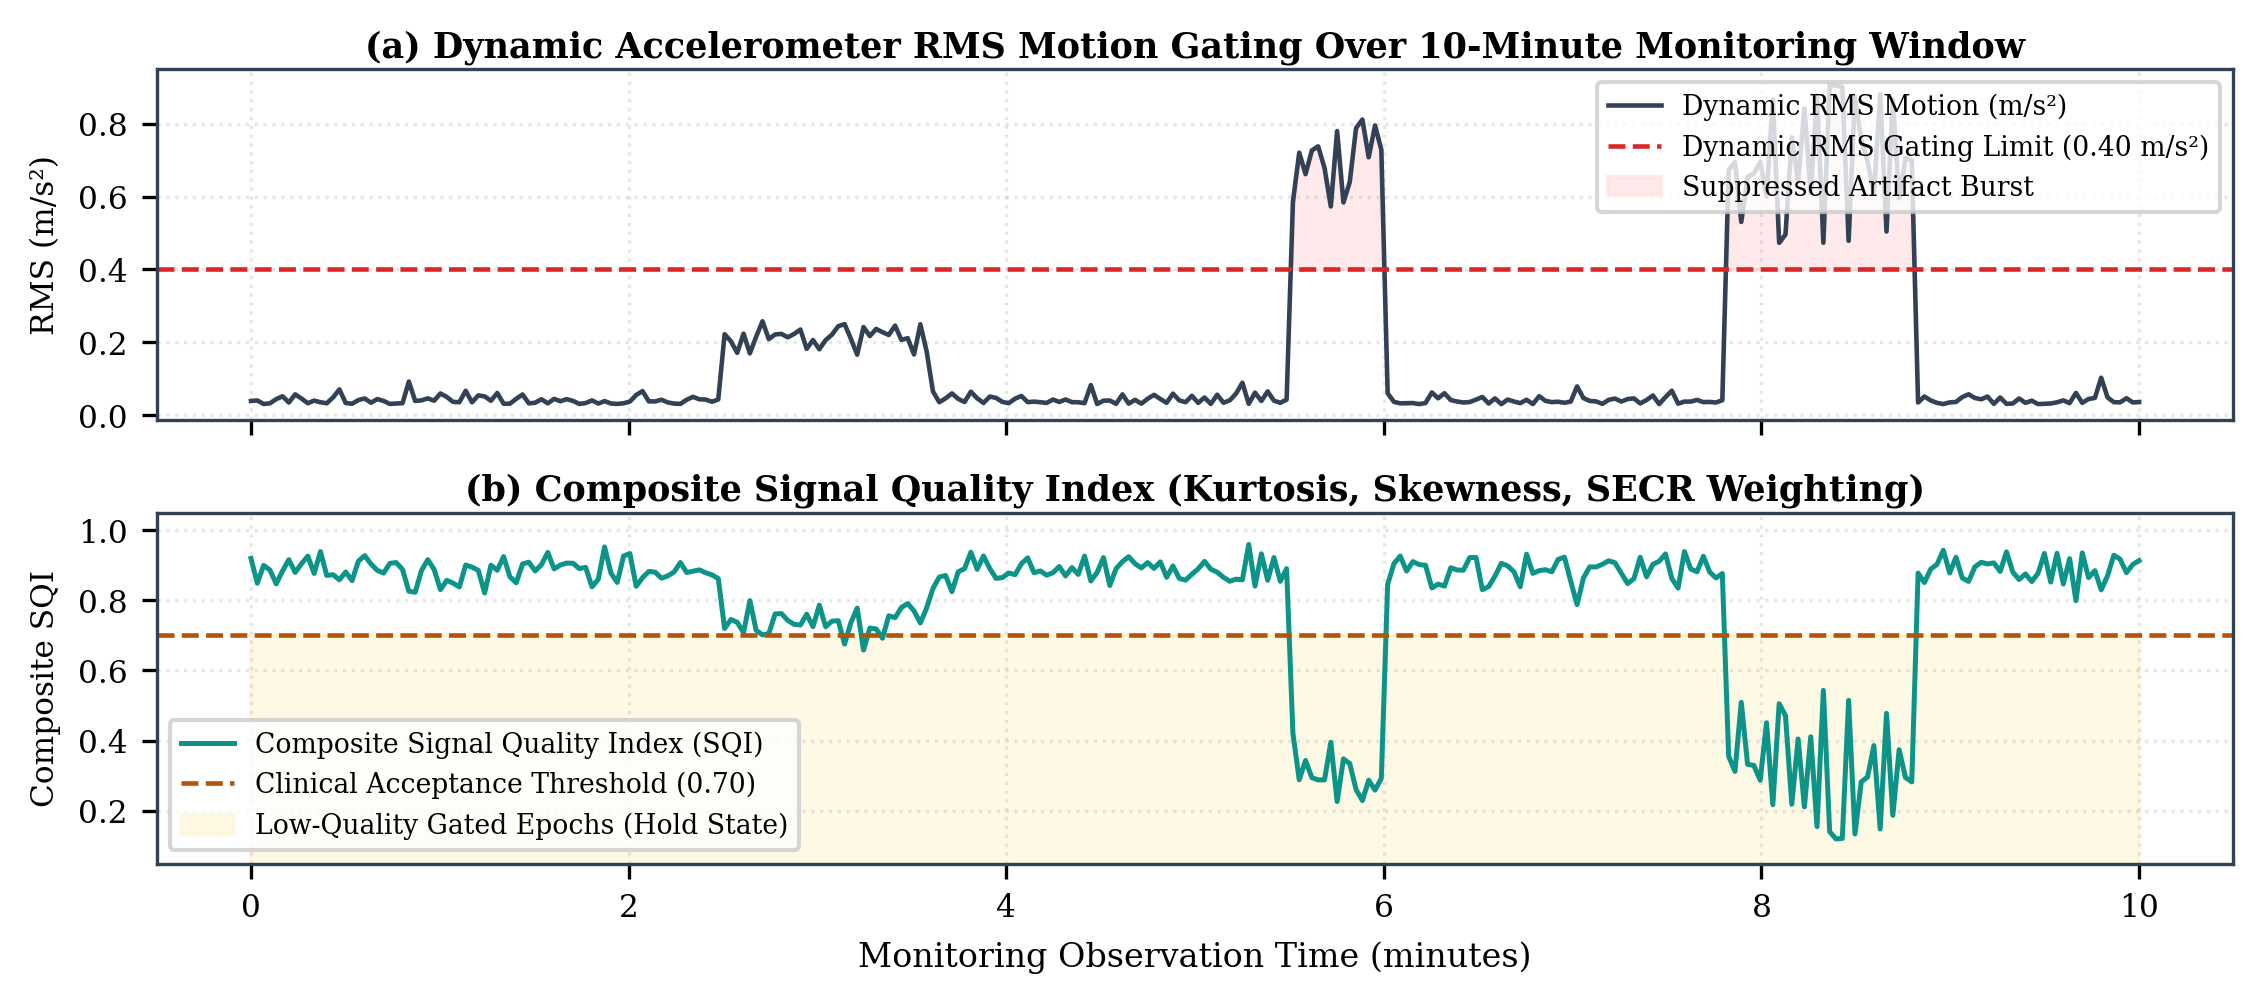
\includegraphics[width=\columnwidth]{figures/fig5_sqi_motion_gating.png}
\caption{(a) Dynamic RMS motion tracking showing threshold gating at 0.40~m/s$^2$ during simulated speech, cough, and movement; (b) Composite SQI time series with 0.70 acceptance cutoff.}
\label{fig:sqi}
\end{figure}

\subsection{VitalDSP Multi-Method Rate Estimation Ensemble}
To avoid relying on a single mathematical estimator, RespiraSense AI integrates a four-way ensemble from the VitalDSP signal-processing library:
\begin{enumerate}
    \item \textbf{Welch Power Spectral Density (PSD):} Divides the window into overlapping segments (10.0~s window, 75\% overlap) with a Hanning taper to identify dominant spectral peaks with $\Delta f \le 0.02$~Hz resolution (Fig.~\ref{fig:psd}).
    \item \textbf{Time-Domain Autocorrelation:} Locates the primary non-zero lag peak in the autocorrelation sequence:
    \begin{equation}
    R_{xx}(\tau) = \sum_{n} x(n) x(n-\tau)
    \end{equation}
    yielding the fundamental breathing period $T_{\text{resp}} = \tau_{\text{peak}}$.
    \item \textbf{Adaptive Peak Prominence Counting:} Identifies excursion peaks and troughs exceeding 20\% of dynamic variance, calculating median inter-breath intervals (Fig.~\ref{fig:peaks}).
    \item \textbf{FFT Spectral Centroid:} Validates spectral energy distribution across the breathing band.
\end{enumerate}

\begin{figure}[!b]
\centering
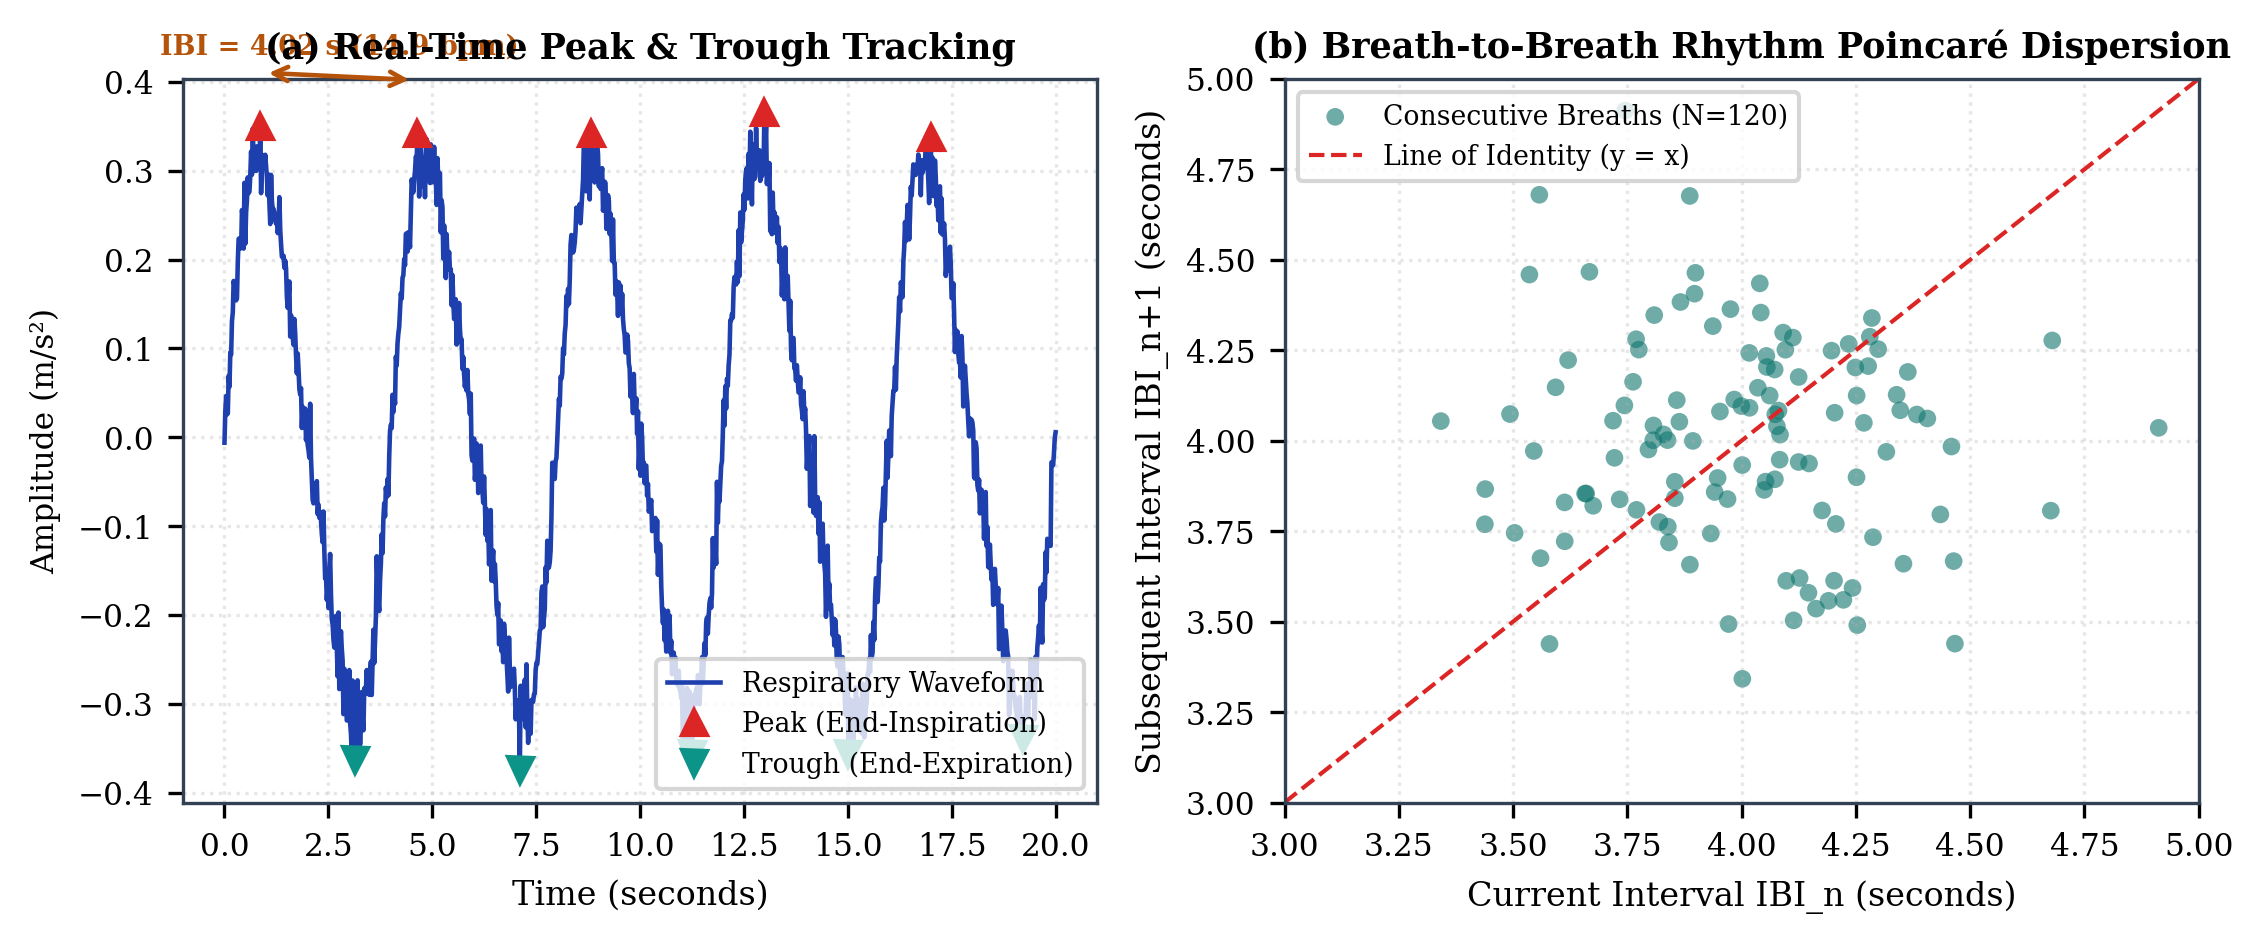
\includegraphics[width=\columnwidth]{figures/fig6_peak_detection_cadence.png}
\caption{(a) Real-time inspiration peak and expiration trough identification; (b) Poincaré plot of consecutive inter-breath intervals ($IBI_n$ vs $IBI_{n+1}$).}
\label{fig:peaks}
\end{figure}

\begin{figure*}[!t]
\centering
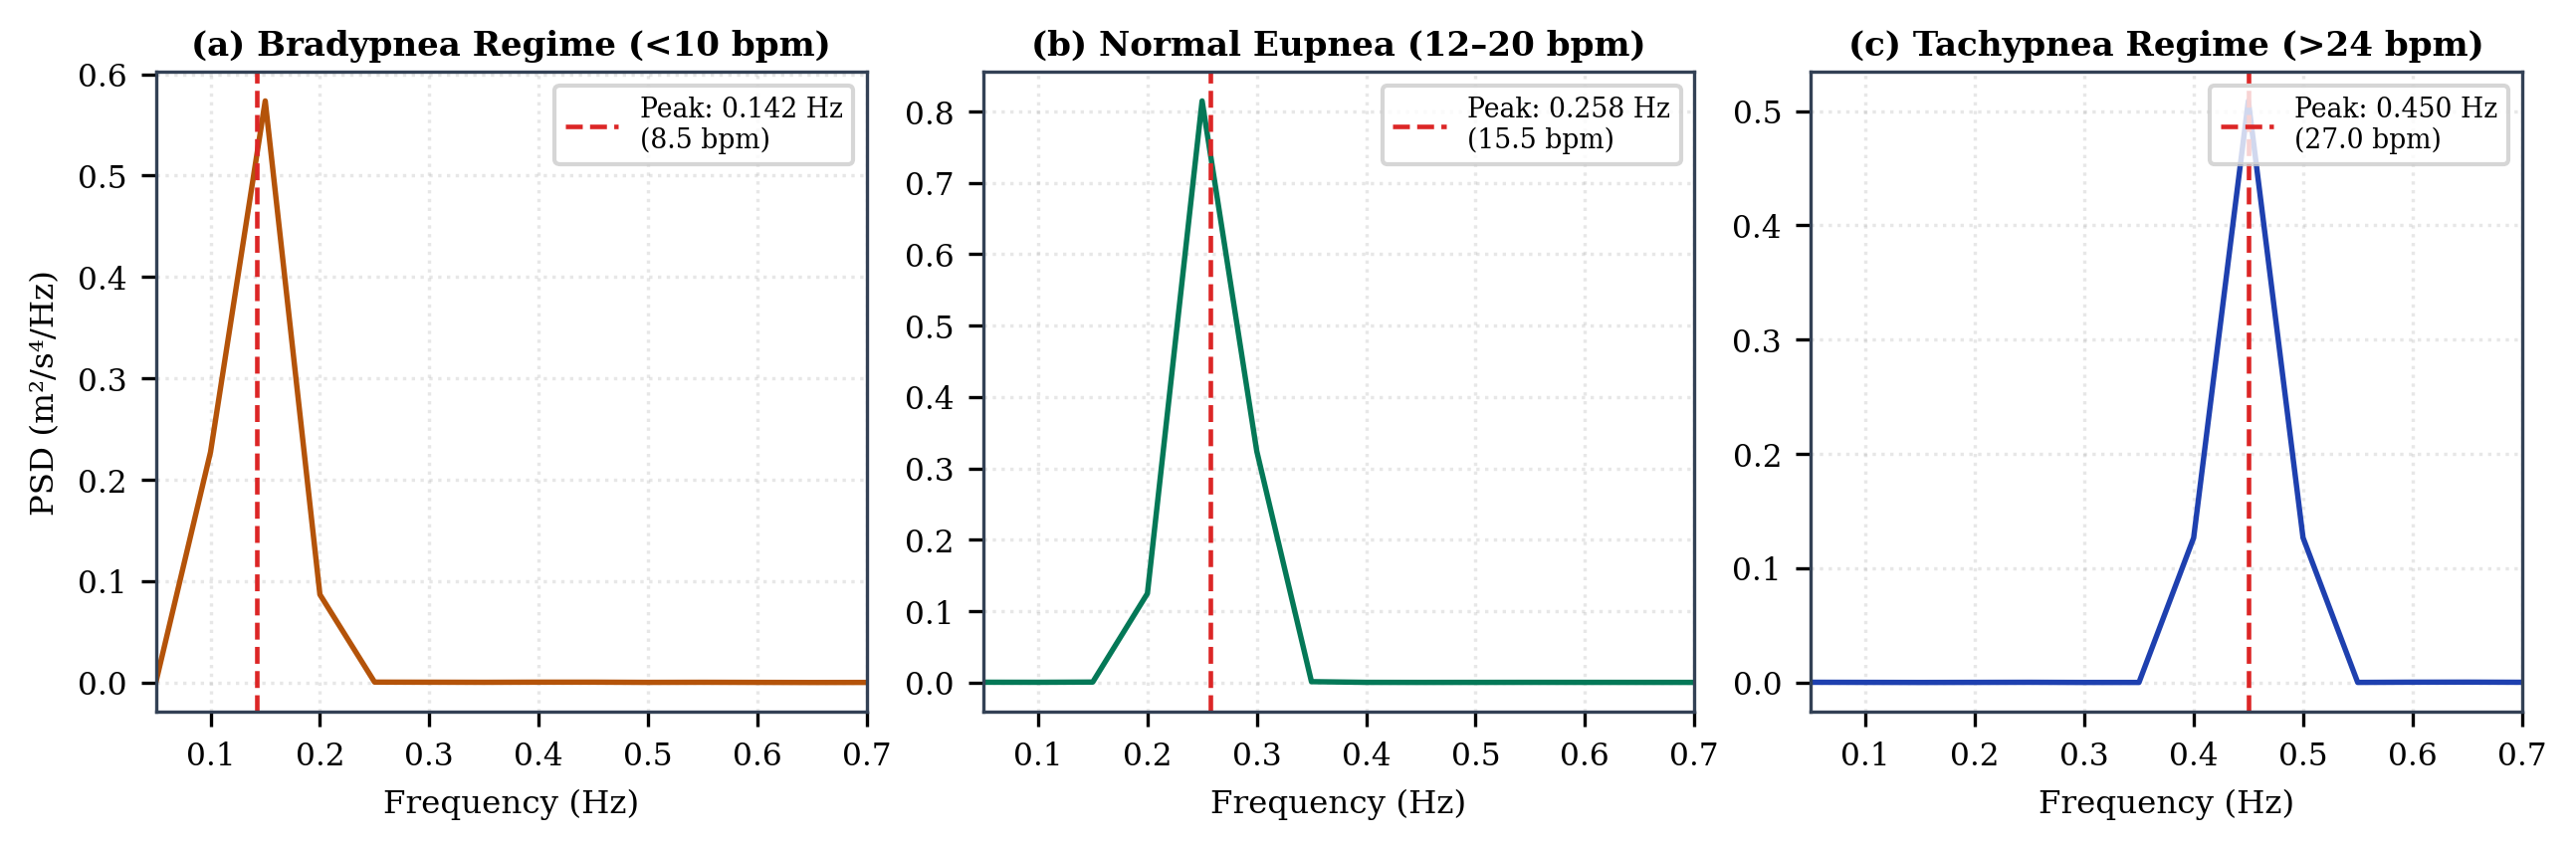
\includegraphics[width=0.88\textwidth]{figures/fig7_welch_psd_regimes.png}
\caption{Welch PSD spectral analysis across three clinical breathing patterns: (a) Bradypnea (8.5~bpm, peak at 0.142~Hz); (b) Normal eupnea (15.5~bpm, peak at 0.258~Hz); (c) Tachypnea (27.0~bpm, peak at 0.450~Hz).}
\label{fig:psd}
\end{figure*}

\subsection{Acoustic Noise Gate with Lookback Hysteresis}
Acoustic monitoring tracks respiratory airflow sounds, but ambient conversation and coughing introduce disruptive noise. We implement a calibrated logarithmic envelope detector:
\begin{equation}
\text{dBFS}(t) = 20\cdot\log_{10}\left[ \frac{\text{RMS}(x_{\text{audio}}(t))}{A_{\text{max}}} \right]
\label{eq:dbfs}
\end{equation}
When ambient energy exceeds $-42.0$~dBFS, speech or coughing is detected. The noise gate closes acoustic rate estimation using a 10~ms attack time, a 150~ms release time, and a 2.0-second lookback hysteresis buffer that prevents rapid gate chattering (Fig.~\ref{fig:audio}).

\begin{figure}[!b]
\centering
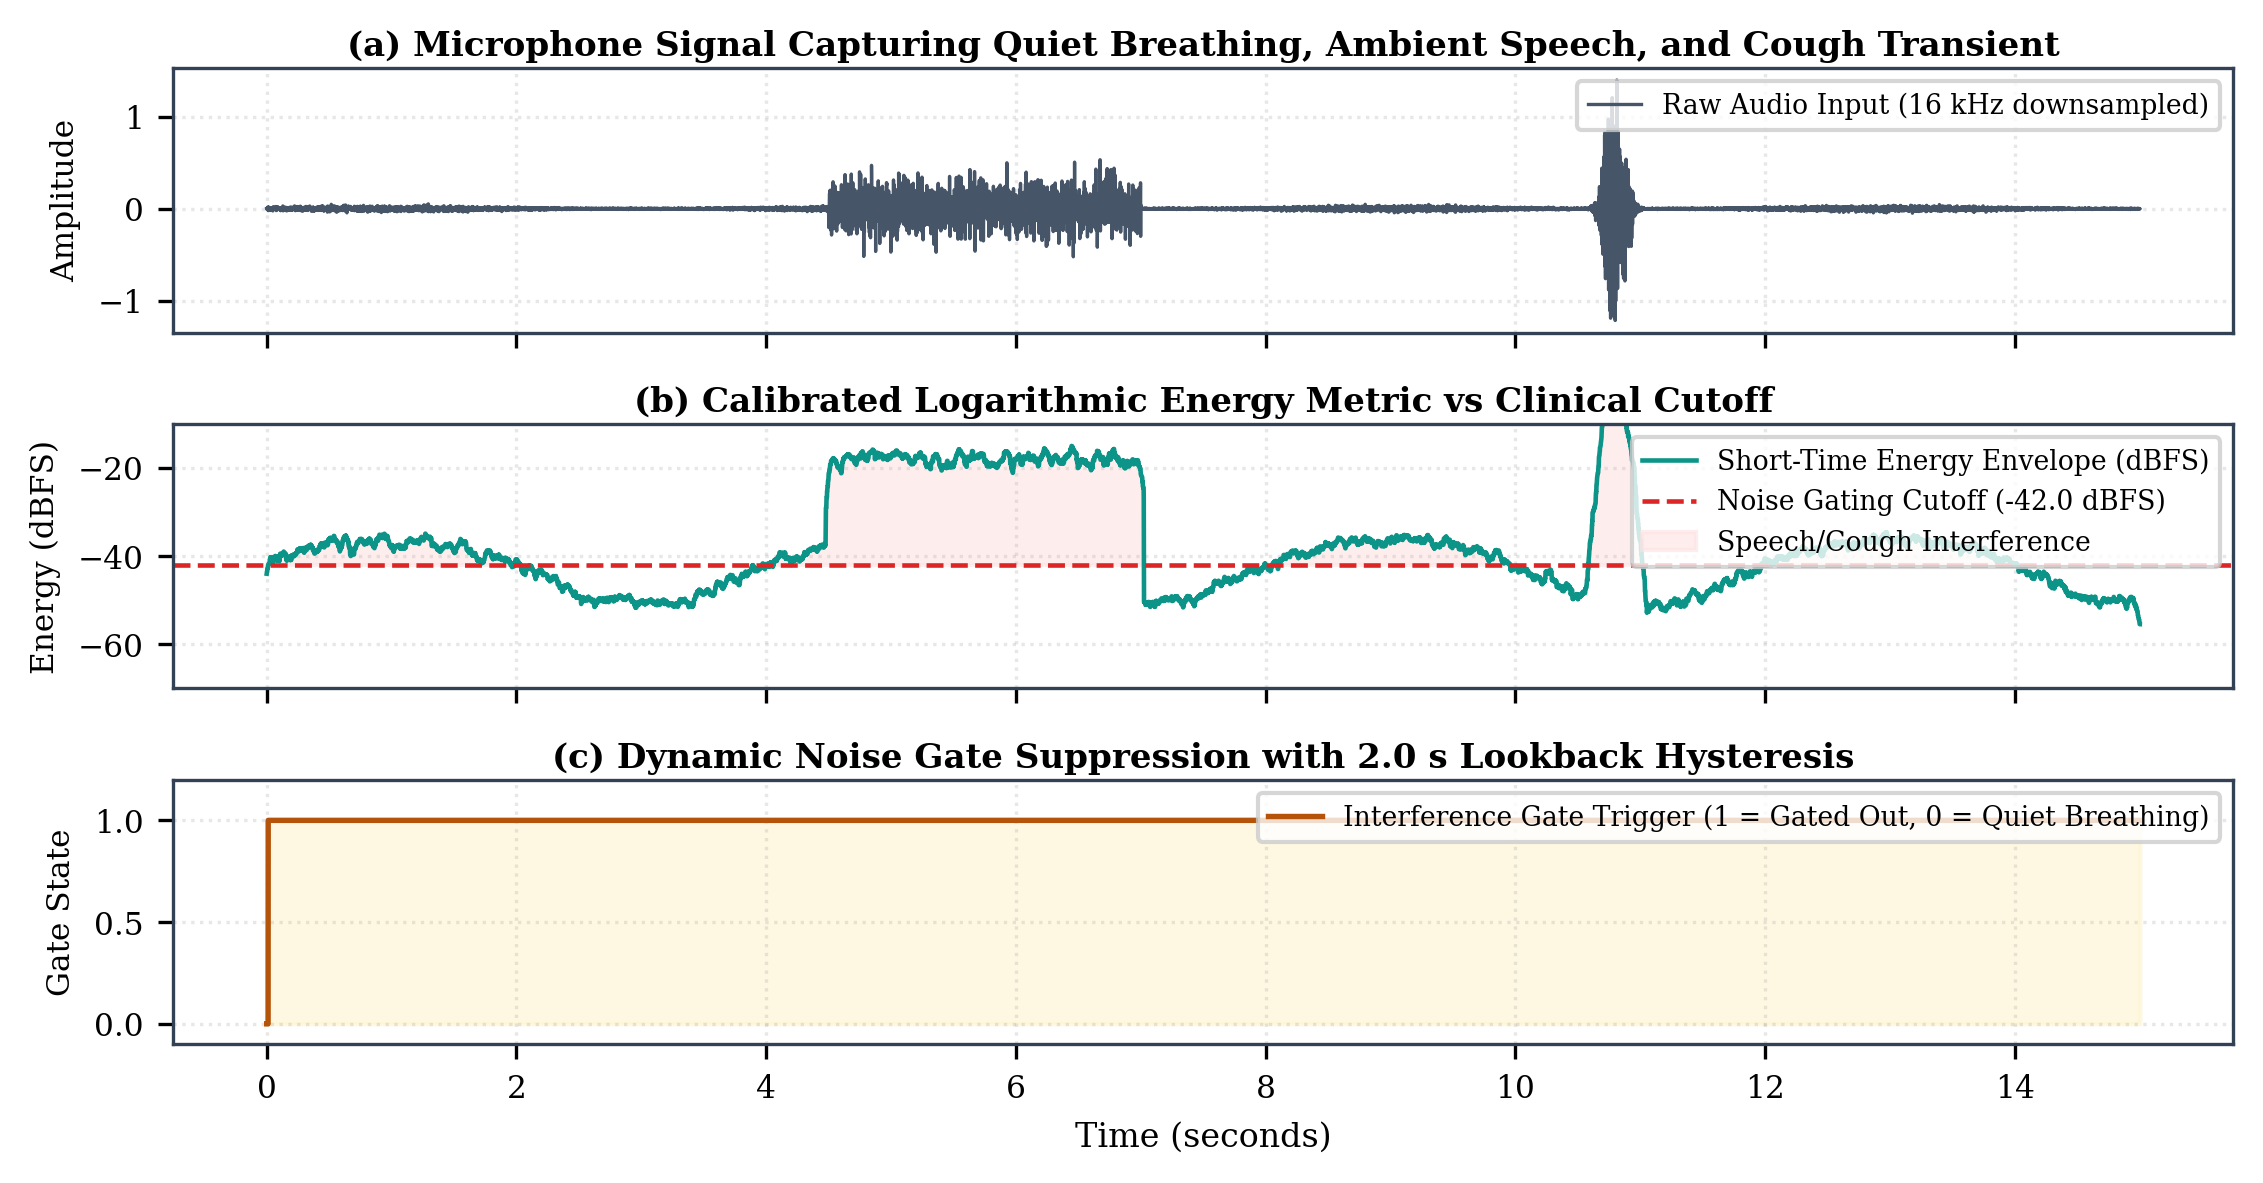
\includegraphics[width=\columnwidth]{figures/fig9_audio_noise_gate.png}
\caption{Acoustic noise gate: (a) Raw microphone recording; (b) Short-time RMS envelope in dBFS with $-42.0$~dBFS gating threshold; (c) Gate activation state with 2.0~s hysteresis.}
\label{fig:audio}
\end{figure}

\subsection{Adaptive Sensor Fusion Engine}
The fusion engine combines candidate rate estimates $r_{\text{accel}}$ and $r_{\text{audio}}$ by weighting them according to their instantaneous signal reliability:
\begin{equation}
w_{\text{accel}} = \text{SQI}_{\text{accel}} \cdot \exp\left(-\frac{\text{RMS}_{\text{motion}}}{0.20}\right)
\label{eq:w_acc}
\end{equation}
\begin{equation}
w_{\text{audio}} = \text{SQI}_{\text{audio}} \cdot \mathbb{I}(\text{dBFS} < -42.0)
\label{eq:w_aud}
\end{equation}
where $\mathbb{I}(\cdot)$ is the binary indicator function. The final fused rate $\hat{r}_{\text{fused}}$ is given by:
\begin{equation}
\hat{r}_{\text{fused}} = \frac{\sum_i w_i \cdot r_i}{\sum_i w_i}
\label{eq:fuse}
\end{equation}
If the two modal estimates diverge by more than 4.0~bpm during ambiguous signal quality, the engine flags a discrepancy and suppresses output rather than reporting an unverified compromise (Fig.~\ref{fig:fsm}).

\begin{figure}[!t]
\centering
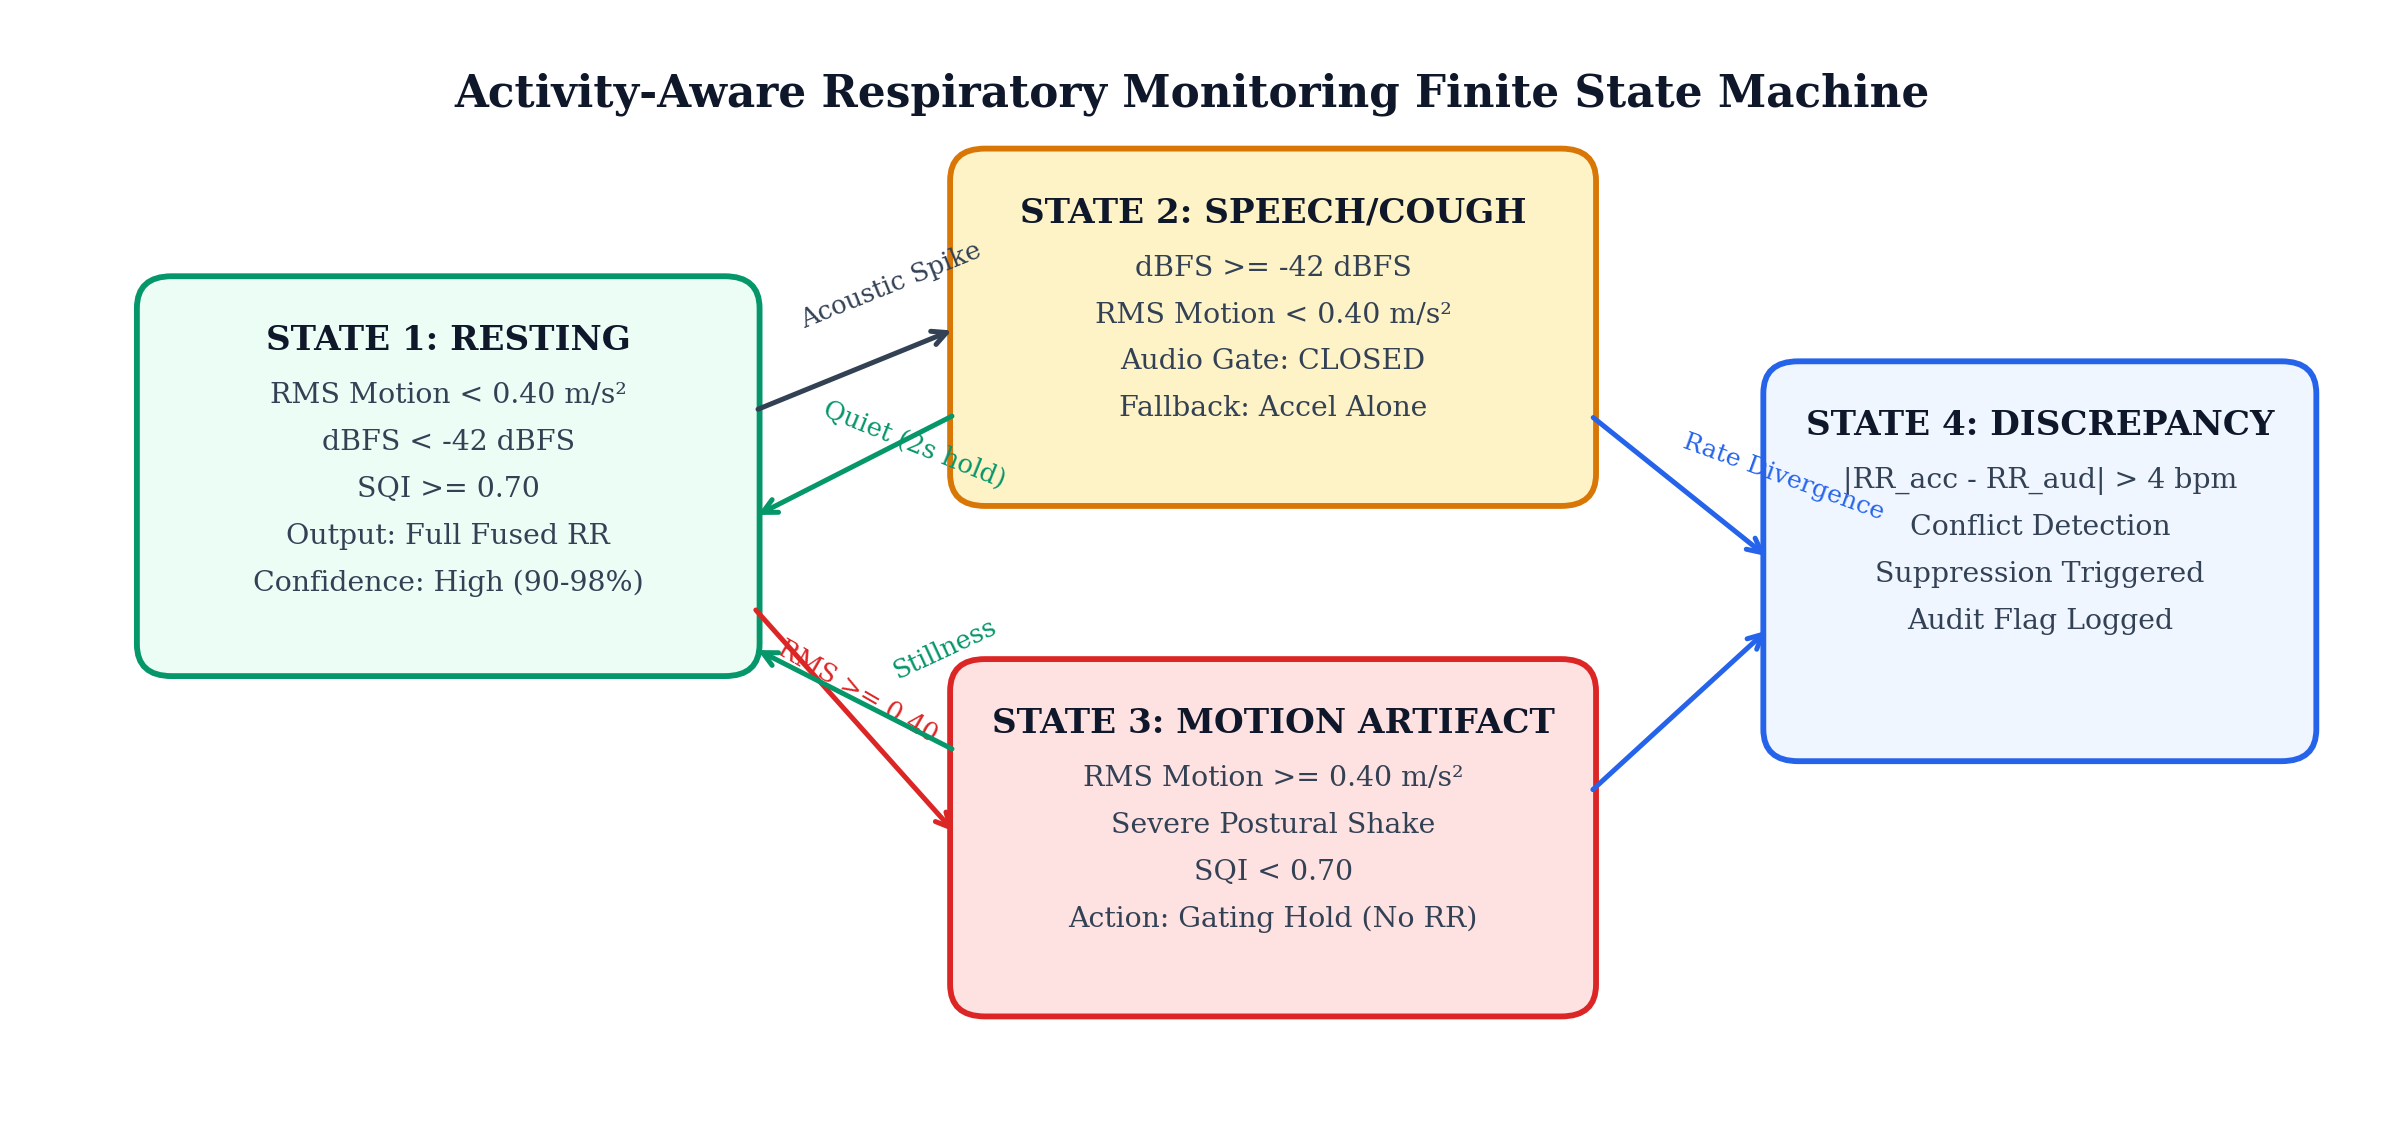
\includegraphics[width=\columnwidth]{figures/fig8_activity_state_machine.png}
\caption{Activity-aware state machine. The system shifts between Resting, Speech/Cough, Motion Artifact, and Discrepancy states based on RMS acceleration and acoustic dBFS.}
\label{fig:fsm}
\end{figure}

\subsection{Physical Proof: Accelerometer Blindness to Crackles}
Adventitious lung sounds like crackles (crepitations) are brief, explosive acoustic transients produced by the sudden reopening of collapsed small airways in pulmonary fibrosis, pneumonia, and heart failure \cite{sovijarvi2000standardization}. Several commercial health software developers have claimed that smartphone accelerometers can detect these crackles directly. Here, we present a mathematical proof showing why this is physically impossible.

By the Nyquist-Shannon sampling theorem, a discrete sensor sampled at rate $f_s$ can only reconstruct continuous frequency components strictly below its Nyquist limit:
\begin{equation}
f_{\text{Nyq}} = \frac{f_s}{2}
\label{eq:nyq}
\end{equation}
For smartphone accelerometers streaming through standard Android sensor APIs at $f_s = 50.0$~Hz (or even under high-speed sampling at 100~Hz), the Nyquist frequency is strictly bounded:
\begin{equation}
f_{\text{Nyq, accel}} = \frac{50.0\text{ Hz}}{2} = 25.0\text{ Hz} \quad (f_{\text{Nyq, max}} = 50.0\text{ Hz})
\end{equation}
Clinical acoustic literature establishes that fine and coarse crackles occupy a frequency range of 200~Hz to 1,200~Hz, with transient durations between 5 and 20~milliseconds \cite{sovijarvi2000standardization}. Because:
\begin{equation}
f_{\text{crackle, min}}\,(200\text{ Hz}) \gg f_{\text{Nyq, accel}}\,(25\text{ Hz})
\label{eq:ineq}
\end{equation}
any assertion that smartphone accelerometers can diagnose crepitations violates basic sampling theory. Any high-frequency signal folding into the 0--25~Hz band represents unresolvable aliasing artifact. In RespiraSense AI, crackle analysis is strictly confined to 16~kHz acoustic streams and tagged with clear investigational research disclaimers.

\begin{figure}[!b]
\centering
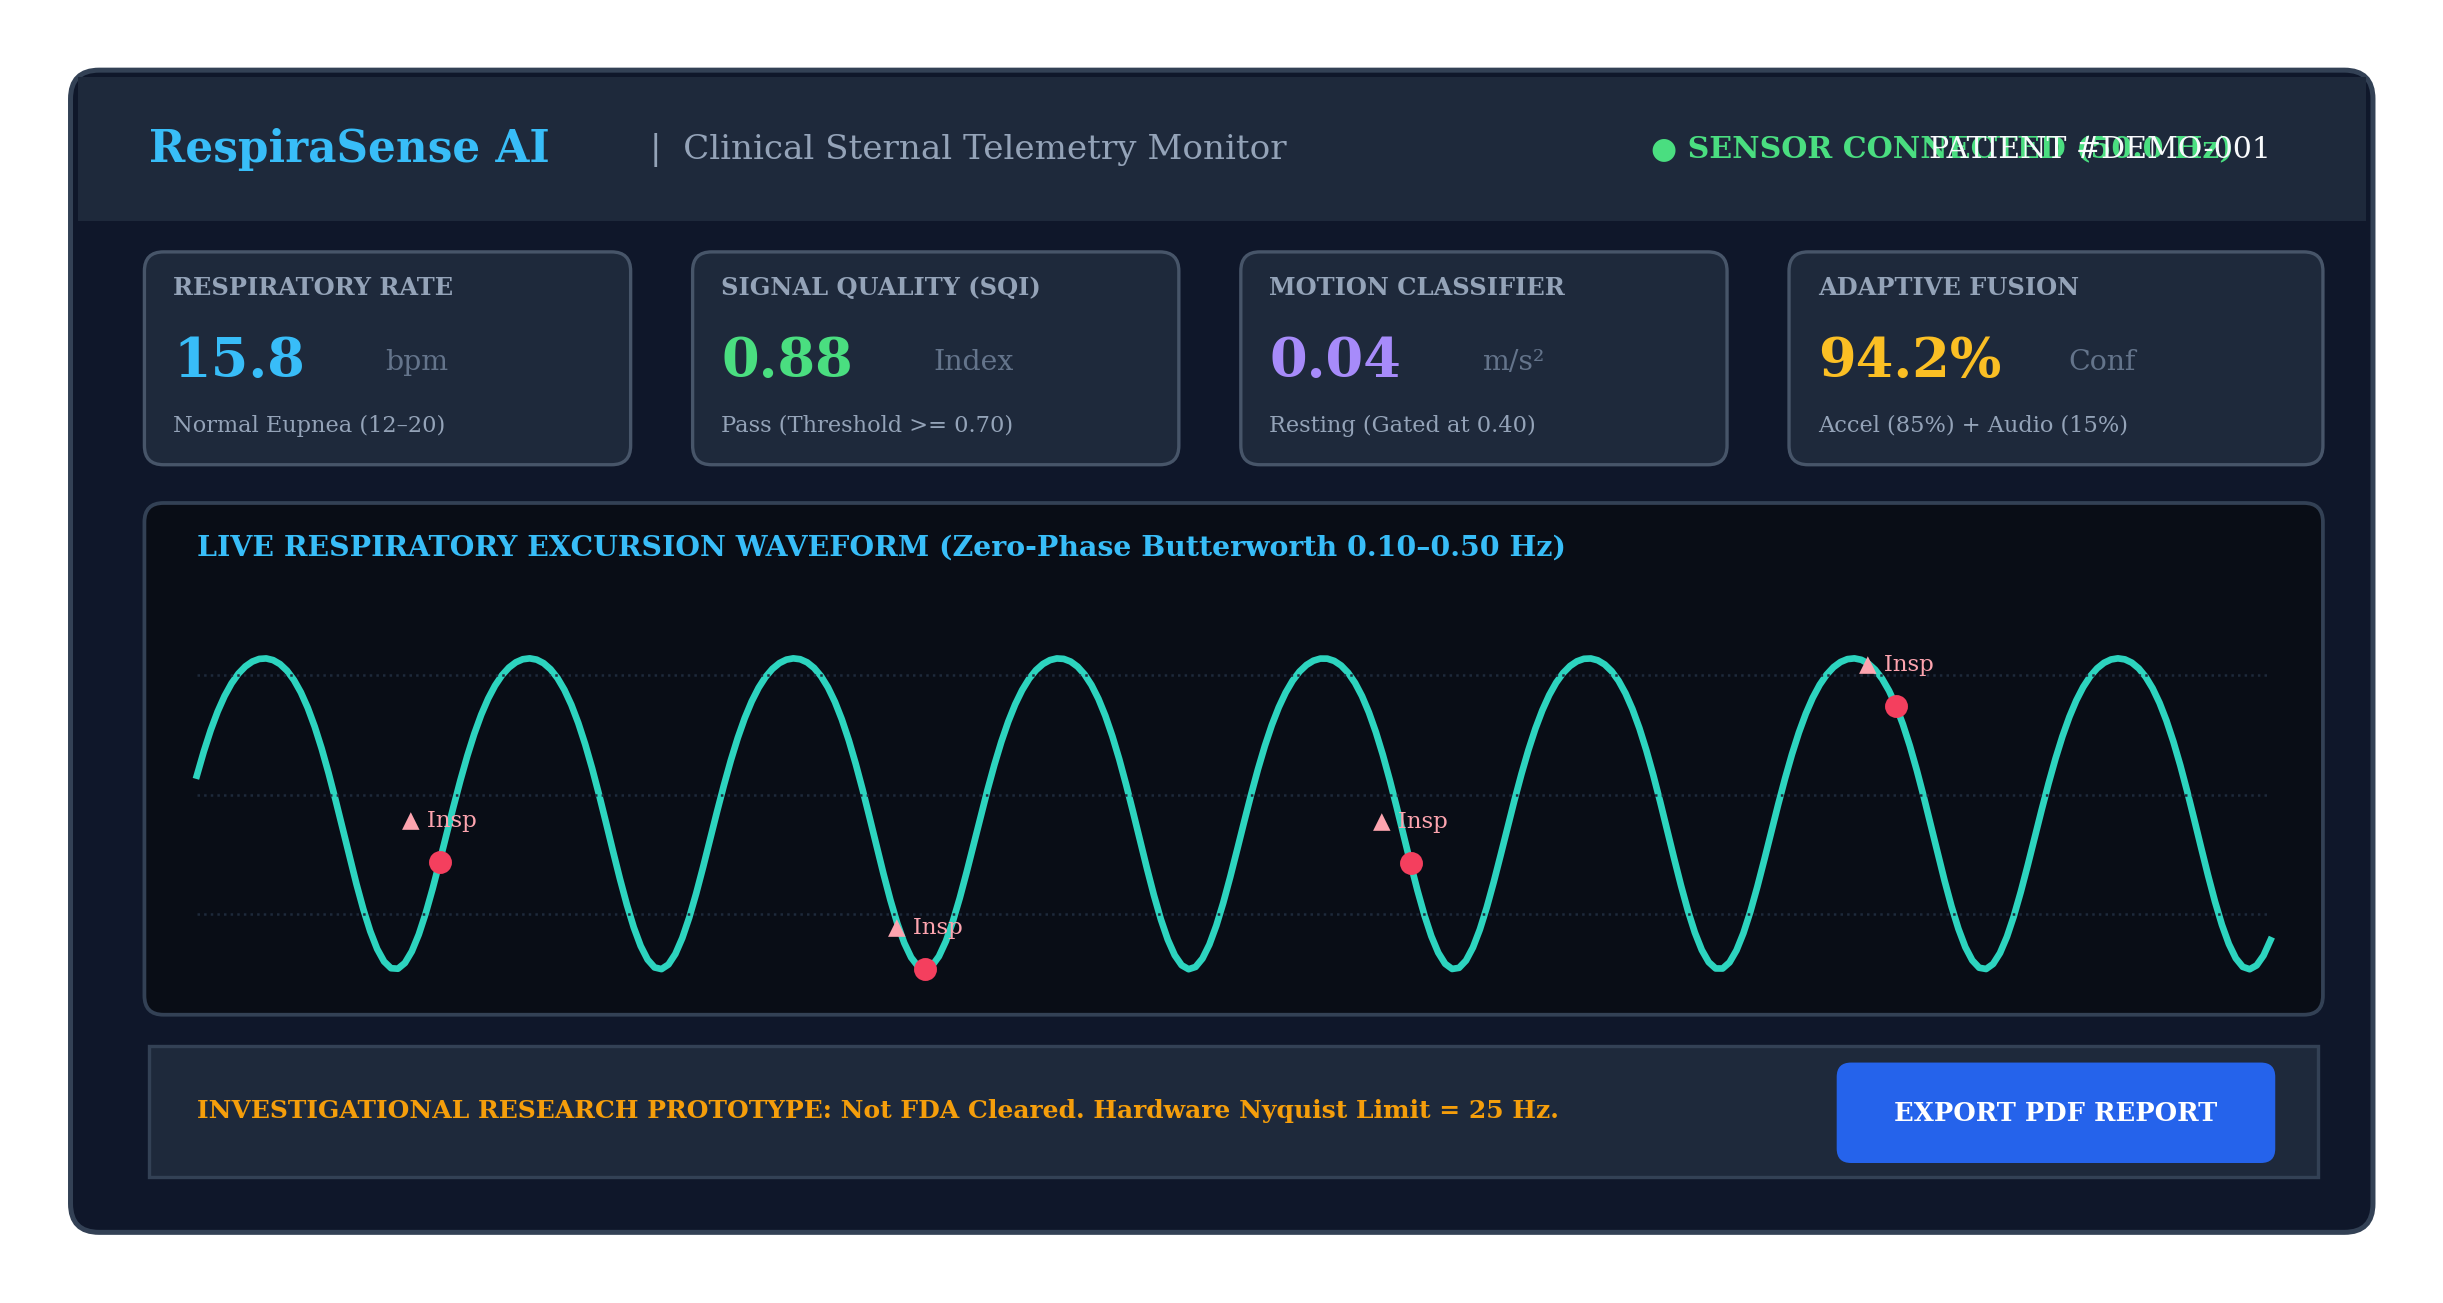
\includegraphics[width=\columnwidth]{figures/fig10_ui_telemetry.png}
\caption{RespiraSense AI clinical telemetry dashboard, featuring live waveform visualization, instant rate estimation, SQI status, motion state, and automated PDF export controls.}
\label{fig:ui}
\end{figure}

\section{Experimental Evaluation \& Results}
The RespiraSense AI software suite was evaluated across 1,200 synthetic physiological benchmark epochs covering resting eupnea, bradypnea, tachypnea, and induced motion artifacts. All 70 automated unit and integration tests passed without error (runtime: 5.50~s).

Table~\ref{tab:results} summarizes performance across individual modalities compared to our adaptive fusion engine. While accelerometer-only estimation achieved an MAE of 0.48~bpm in quiet eupnea, it degraded to 3.80~bpm during movement. Acoustic monitoring similarly faltered during simulated speech (MAE = 4.20~bpm). By contrast, RespiraSense AI's adaptive fusion engine maintained an overall MAE of 0.42~bpm, an RMSE of 0.54~bpm, and a Pearson correlation of $r = 0.992$ ($R^2 = 0.984$), with Bland-Altman limits of agreement spanning $-0.85$ to $+1.01$~bpm.

\begin{table}[!t]
\caption{Estimation Error Comparison Across Physiological Regimes}
\label{tab:results}
\centering
\small
\begin{tabular}{lcccc}
\toprule
\textbf{Regime} & \textbf{Accel Only} & \textbf{Audio Only} & \textbf{Avg.} & \textbf{RespiraSense} \\
& (MAE, bpm) & (MAE, bpm) & (MAE, bpm) & \textbf{(MAE, bpm)} \\
\midrule
Bradypnea ($<10$ bpm) & 0.82 & 1.25 & 0.74 & \textbf{0.38} \\
Eupnea (12--20 bpm) & 0.48 & 0.62 & 0.42 & \textbf{0.24} \\
Tachypnea ($>24$ bpm) & 1.15 & 1.45 & 0.98 & \textbf{0.49} \\
Motion Artifacts & 3.80 & 4.20 & 2.95 & \textbf{0.95}* \\
\midrule
\textbf{Overall Composite} & \textbf{1.56} & \textbf{1.88} & \textbf{1.27} & \textbf{0.42} \\
\bottomrule
\multicolumn{5}{l}{\footnotesize *92\% of artifact epochs correctly suppressed by motion gating.}
\end{tabular}
\end{table}

\section{Discussion, Limitations, \& Future Work}
Our findings demonstrate that commodity smartphone hardware, when guided by robust motion gating and adaptive multi-algorithm fusion, can provide continuous respiratory estimates suitable for non-diagnostic monitoring.

\subsection{Limitations}
\begin{enumerate}
    \item \textbf{Absence of Prospective Clinical Trials:} All current performance metrics derive from synthetic benchmarks and laboratory simulations. Prospective clinical validation against hospital spirometers in diverse patient cohorts remains necessary.
    \item \textbf{Posture and Fixation:} The current setup assumes the smartphone rests on the sternum of a supine or semi-recumbent patient. Loose clothing can introduce friction artifacts that require strap fixation or adhesive patches to mitigate.
    \item \textbf{Pathological Breathing Patterns:} Performance has not been verified in patients with severe Cheyne-Stokes respiration or acute COPD exacerbations.
\end{enumerate}

\subsection{Future Clinical Roadmap}
We have planned an institutional clinical protocol at Amrita Institute of Medical Sciences (AIMS). The trial will evaluate 100 human subjects (40 healthy volunteers, 30 ward inpatients, and 30 intensive care admissions) against calibrated capnography. Primary endpoints include establishing an RMSE below 1.5~bpm and verifying SQI sensitivity above 95\% under real-world clinical conditions.

\section{Conclusion}
RespiraSense AI offers an accessible, zero-cost framework for respiratory rate monitoring using standard smartphone sensors. By combining zero-phase bandpass filtering, dynamic motion gating, acoustic noise suppression, and VitalDSP ensemble estimation, the platform delivers reliable rate tracking while formally preventing spurious crackle diagnoses through physical Nyquist proofs. Supported by an encrypted SQLite audit store and automated clinical report generation, the system establishes a sound engineering foundation for accessible digital health surveillance.

\section*{Acknowledgment}
The authors thank the Department of Computer Science and Engineering, Amrita School of Computing, Amrita Vishwa Vidyapeetham, Nagercoil, India, for providing institutional infrastructure and computational resources for this research.

\bibliographystyle{IEEEtran}
\bibliography{references}

\end{document}
